\section{单调栈}
\par \noindent 给出一个01矩阵,求全1子矩阵的个数。
\begin{enumerate}
\item 按行枚举子矩阵的底边,然后求以该行为底边的子矩阵的个数。
\item 预处理 int H[N][N]:向上最大扩展全1的长度,然后就可以用单调栈解决。
\item 为了避免计算重复,单调栈时左闭右开即可。
\end{enumerate}

\begin{figure}
        \centering
        \par 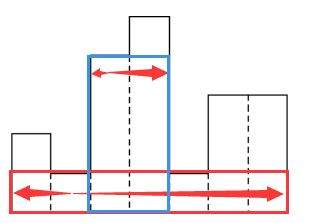
\includegraphics[width=10cm]{images/stack.png}
\end{figure}

\par \noindent 按照上述思想也能够求最大子矩形的面积。
~\\
\par \noindent 注意此做法能够优化到O(矩形1的数量),因为可以直接枚举同一行的1的位置,考虑该行相邻列都是1的情况此时计算一次答案。【按照矩形的分布计算,因为一个位置是0就可以隔断子矩形】

\begin{minted}{c++}
#include <bits/stdc++.h>

using namespace std;
const int N = 1e3 + 5;
using ll = int64_t;
int n, m, a[N][N];
int H[N][N]; // 向上最大扩展全1的长度
ll calc(int *h, int k) {//计算矩形个数 下标[0, k)
    stack<int> s;
    vector<int> l(k), r(k);
    for (int  i = k - 1; i >= 0; i--) {
        while (!s.empty() && h[i] <= h[s.top()]) l[s.top()] = i, s.pop();
        s.push(i);
    }
    while (!s.empty()) l[s.top()] = -1, s.pop();
    
    for (int  i = 0; i <= k - 1; i++) {
        while (!s.empty() && h[i] < h[s.top()]) r[s.top()] = i, s.pop();
        s.push(i);
    }
    while (!s.empty()) r[s.top()] = k, s.pop();
    ll res = 0;
    for (int  i = 0; i <= k - 1; i++)  res += (ll)h[i] * (i - l[i]) * (r[i] - i);
    return res;
}
int main() {
    scanf("%d%d", &n, &m);
    for (int i = 1; i <= n; i++) 
        for (int j = 1; j <= m; j++) 
            scanf("%d", &a[i][j]);
    ll ans = 0;
    for (int i = 1; i <= n; i++)  {
        for (int j = 1; j <= m; j++) {
            if (a[i][j])
                H[i][j] = H[i-1][j] + 1;
            else
                H[i][j] = 0;
        }
        ans += calc(H[i] + 1, m); // 每一行算一次
    }
    printf("%lld\n", ans);
    return 0;
}
/**
2 2
0 1
1 1 
子矩形数量是5
**/
\end{minted}